\section{Probleme}
Bei der Bearbeitung der gegebenen Aufgabenstellung der Projektgruppe haben einige Probleme zu Verzögerungen geführt, welche sich auf die endgültige Funktionalität des Endprodukts ausgewirkt haben.

\subsection{Stabilität des Skeletts}
Das Hauptproblem für die Animatoren-Teilgruppe, welche Hauptsächlich mithilfe von maschinellem Training eine beliebige Kreatur zum laufen bringt, liegt in der Kreaturenstabilität. Zum Anfang der Arbeitsphase wurde die bestehende Walker-Umgebung von Unity analysiert und auf Basis der in dieser Umgebung vorhandenen Kreatur die ersten Tests erstellt. Hierbei konnte verifiziert werden, dass die neu entwickelte Trainingsumgebung funktioniert und die grundlegenden Einstellung zu funktionierenden Ergebnissen führen. Als danach die ersten prozedural generierten Kreaturen eingesetzt wurden, kam es zu einer Vielzahl von Problemen, welche durch andere Defizite in verschiedene Bereichen verstärkt wurden. In Abbildung \ref{fig:explodierendeKreatur} ist eine Kreatur aus der Anfangsphase der PG dargestellt. Diese Figur konnte nicht trainiert werden, da ihre einzelnen Teile durch die im Folgenden beschriebenen Probleme instabil waren.

\begin{figure}
	\centering
	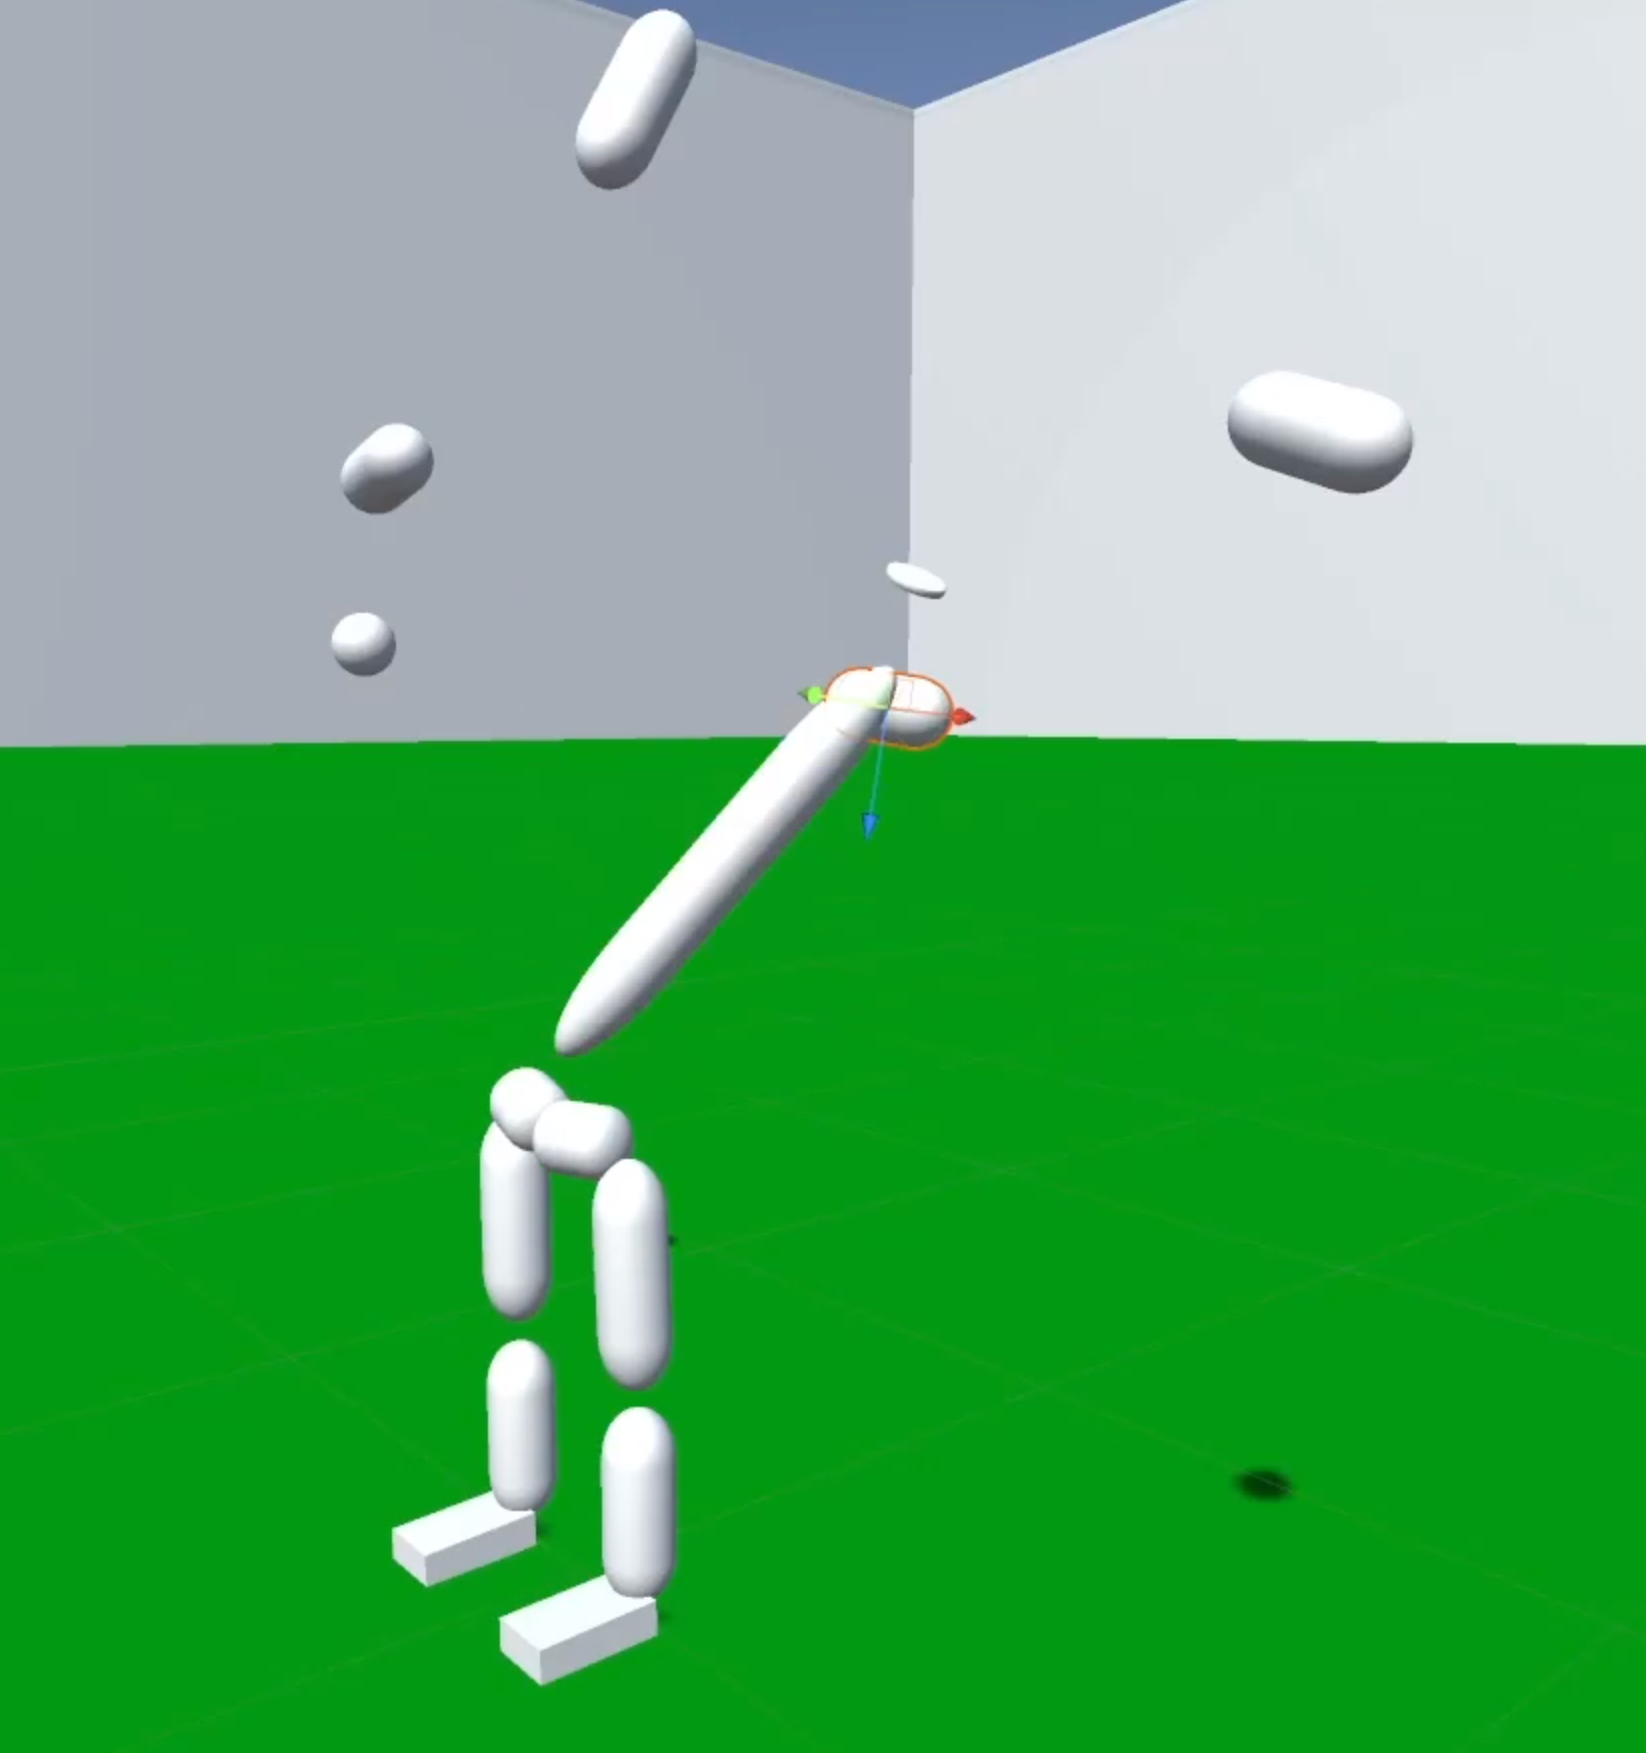
\includegraphics[width=0.5\linewidth]{resources/img/Discord_XmWjop66BU}
	\caption[Beispiel explodierende Kreatur]{Beispiel einer durch fehlerhaften Einstellungen zerstörte Kreatur.}
	\label{fig:explodierendeKreatur}
\end{figure}

\subsubsection{Dokumentation} % Nils
Die meisten Projektgruppenmitglieder hatten vor der PG wenig Erfahrungen mit Unity. Deshalb ist die Dokumentation von Unity eine der wichtigsten Quellen für die Umsetzung der einzelnen Teilprojekte. Die Unity-Dokumentation\footnote{\url{https://docs.unity3d.com/Manual/index.html}} ist Online frei einsehbar für die verschiedenen Versionen der Grafik-Engine. Dabei ist problematisch, dass insbesondere in den Teil zur Physik-Engine oder neueren Pakete ist, welche noch nicht den Vorschau-Status verlassen haben, deutliche Formulierungen fehlen. Ein Beispiel dafür ist die Hilfestellung zur Ragdoll-Stabilität. In einen Nebensatz\footnote{Zu finden auf dieser Unterseite der Dokumentation \url{https://docs.unity3d.com/Manual/RagdollStability.html}} wird erwähnt, dass ein zu großer Massenunterschied zwischen zwei direkt verbundenen Elementen zu unruhigen Ragdolls führen kann. In der Praxis bedeutet dies, dass die generierten Kreaturen bei jegliche Krafteinwirkung explodieren. Eine Fehler-findung und -behebung dieses Problems hat mehrere Wochen gedauert, da die Auswirkungen nur in sehr abgeschwächter Form beschrieben wurden.

Ein weiteres Beispiel ist der \emph{Solver Type}\footnote{Die Komponente der Physikumgebung, welche die Berechnungen für die Kollisionserkennung durchführt.}, welche auf \emph{Projected Gauss Seidel} oder \emph{Temporal Gauss Seidel} gesetzt werden kann. Für das Training wurde in der Anfangsphase versucht jeweils die besten Einstellungen von Unity zu verwenden, was nach Dokumentation die zweitere Option sein sollte. In Gegensatz zu der Dokumentation warnen mehrere Internetquellen\footnote{Siehe beispielsweise das zum PG-Zeitpunkt \href{https://www.youtube.com/watch?v=aZ1zc6zZ61E}{erste Google-Ergebnis}} vor dieser Einstellung. Ein nicht repräsentativer Test hat dies für unsere Kreaturen bestätigt, weshalb im weiteren Verlauf \emph{Projected Gauss Seidel} genutzt wurde. Ein Hinweis, dass \emph{Temporal Gauss Seidel} problematische Ergebnisse produzieren kann, fehlt zum Zeitpunkt des Projetgruppenberichts weiterhin in der Dokumentation.

Insgesamt gab es weitere Beispiele, wie zum Beispiel bei dem \texttt{com.unity.ai.navigation}-Paket \footnote{Eine Dokumentation ist \href{https://docs.unity3d.com/Packages/com.unity.ai.navigation@1.0/manual/NavMeshSurface.html}{hier} zu finden} bei welchem die unterstützten Unity-Versionen unklar ist, welche zusammen zu viel Recherchearbeit geführt haben und deshalb die Bearbeitung der Kernaufgaben verzögert haben.

\subsubsection{Organisatorische Probleme}
Ein weiterer Teilbereich, der zu Verzögerung in den Arbeitsablauf der Animatorenteilgruppe geführt hat, ist organisatorischen Problemen zu zuschrieben. Einige der größten Hindernisse sind die starke Abhängigkeit von den Animatoren und Generatoren, veralte Rechenhardware und fehlender Vorkenntnisse.

Das erste Problem kann wie folgt beschrieben werden. Immer wenn die Änderung an der Kreatur nötig waren, musste das für die Generierung verantwortliche Paket angepasst werden. Inklusive der Kommunikation und der dafür benötigten Arbeitszeit dauerte dies ungefähr eine Woche. In diesen Phasen konnte das Training häufig nicht fortgesetzt werden, da die Kreaturen zu große Fehler hatten. In die andere Richtung konnten die Generatoren nicht weiterarbeiten, da diese auf Feedback von den Trainingsversuchen gewartet haben.

Verstärkt wurde dies durch das zweite Problem. Da LIDO von der ganzen Universität genutzt wird, kann es einige Stunden bis Tage dauern, bis eine Aufgabe abgearbeitet wird. Inklusive der Berechnungszeit des Auftrags konnten so 2 aufeinanderfolgende Experimente gestartet werden je Woche. Da insbesondere in der Mitte der Projektgruppe die Fehler nicht bekannt waren, dauerte das Finden dieser dadurch besonders lange. 
Zusätzlich zu der Wartezeit ist die Rechendauer eines Auftrags auf LIDO für Studenten eingeschränkt. Ein Knoten mit Grafikkarte kann 2 Tage lang reserviert werden. Bei den finalen Training auf einen Knoten des Lehrstuhls stellt sich heraus, dass diese Zeit nicht ausreichend ist, um das (lokale) Maximum der Belohnungsfunktion zu erreichen. Theoretisch wäre ein Fortsetzen der Trainingsaufgabe möglich, führt aber zu eine weiteren Wartezeit auf einen Knoten und Verfälschungen der Trainingsergebnisse durch nicht perfekt zurückgesetzten Parameter des Trainings. 
Des Weiteren stellte sich heraus, dass das Training auf den alten Knoten signifikant länger dauert, als auf den aktuell ausgestatteten Rechenknoten des Lehrstuhls. Ein Trainingsschritt auf den öffentlichen Knoten dauert um die $160 \si{\sec}$  und auf den Lehrstuhlknoten $60 \si{\sec}$. Dies führt zu einer 3-Fachen Wartedauer während der meisten Experimente.

Zuletzt fehlten insbesondere bei dem maschinellen Lernen viele Vorkenntnisse. Das zu Beginn der PG gehaltene Seminar beschäftigte sich mit den eigentlich genutzten Algorithmen, hat aber keine Übersicht über die Forschung im Bereich des physikalischen Laufens gegeben. Hier wurde später \cite{Geijtenbeek2012} genutzt, welches aufgrund des Erscheinungsjahrs kein Überblick für Netzwerkbasierte-Lernmethoden gibt. Eine Einschätzung von weiteren Papieren war dadurch erschwert. Weiterhin beziehen sich viele Arbeiten auf andere Physikumgebgungen, nutzen Imitation zum Lernen oder nutzen explizite Designcharakteristiken der Kreaturen aus\cite{Mourot2022}.

Insgesamt führten die Probleme häufig zu Arbeitsphasen in den die Animatorengruppe oder Generatoren keine neuen Ergebnisse produzieren konnten. In dieser Zeit wurde versucht zukünftige Aufgaben wie beispielsweise eine Generalisierung der Belohnungsfunktionen, eine stärkere anpassbare Trainingsumgebung oder Zusatzfunktionen wie ein unebener Boden. Durch die grundlegenden Probleme bei der Stabilität konnte am Ende keine dieser Erweiterungen fertiggestellt werden.